% abnTeX2: Modelo de Trabalho Academico  em conformidade com ABNT NBR 14724:2011
% http://www.abntex.net.br/

% Customização Dept. Engenharia Elétrica UFF
% Autor: Bernardo Albuquerque (Adaptado da Prof. Malú Grave e Jonas Alessi)
% Versão: 15 de Janeiro de 2025.

% Edição: VSCode (LaTeX Workshop + LaTeX Utilities)
% Programas necessários: MiKTeX, Strawberry Perl, Inkscape
% Codificação: UTF-8
% LaTeX: abnTeX2
% ----------------------------------------------------------------------------------------------------------------------

\documentclass[
  12pt,				                                                                                                          % Tamanho da fonte	
  oneside,                                                                                                              % Não imprimir em verso e anverso, oposto do twoside 
  a4paper,			                                                                                                        % Tamanho do papel. 
  chapter = Title,		                                                                                                  % Títulos de capítulos convertidos em letras maiúsculas
  section = Title,		                                                                                                  % Títulos de seções convertidos em letras maiúsculas
  subsection = Title,	                                                                                                  % Títulos de subseções convertidos em letras maiúsculas
  english,			                                                                                                        % Idioma adicional para hifenização
  brazil,			                                                                                                          % O último idioma é o principal do documento
  sumario = tradicional
  ]{abntex2-uff}

% abnTeX2: Modelo de Trabalho Academico  em conformidade com ABNT NBR 14724:2011
% http://www.abntex.net.br/

% Customização Dept. Engenharia Elétrica UFF
% Autor: Bernardo Albuquerque (Adaptado da Prof. Malú Grave e Jonas Alessi)
% Versão: 15 de Janeiro de 2025.

% Edição: VSCode (LaTeX Workshop + LaTeX Utilities)
% Programas necessários: MiKTeX, Strawberry Perl, Inkscape
% Codificação: UTF-8
% LaTeX: abnTeX2
% ----------------------------------------------------------------------------------------------------------------------
\usepackage{cmap}                																						% Mapear caracteres especiais no PDF
\usepackage[scaled = .85]{zi4}
\usepackage[scaled = .82]{DejaVuSerif}
\usepackage[T1]{fontenc}         																						% Selecao de codigos de fonte
\usepackage[utf8]{inputenc}      																						% Codificacao do documento (conversão automática dos acentos)
\usepackage{lastpage}            																						% Usado pela Ficha catalográfica
\usepackage{indentfirst}         																						% Indenta o primeiro parágrafo de cada seção
\usepackage{color}               																						% Controle das cores
\usepackage{graphicx}            																						% Inclusão de gráficos
\usepackage{tocloft}
\usepackage[newfloat]{minted}
\usepackage{amsfonts}            																						% Símbolos
\usepackage[none]{hyphenat}      																						% Sem separação de sílabas
\usepackage{pdfpages}            																						% Acrescentar pdf ficha bibliográfica
\usepackage{caption}
\usepackage{titlesec}            																						% Modificar títulos
\usepackage{svg}                 																						% Pacote para incluir imagens svg
\usepackage{lipsum}              																						% para geração de dummy text
\usepackage[brazilian, hyperpageref]{backref}  																			% Paginas com as citações na bibliografia
\usepackage{enumitem}
	\setitemize[0]{itemindent=0.4cm, itemsep=0pt}
	\setenumerate[0]{itemindent=0.5cm, itemsep=0pt}
\usepackage[alf,
abnt-emphasize=bf,		 		 																						      % destaca o título da obra em negrito
abnt-url-package=none,			 																						    % Utiliza o pacote url
abnt-repeated-title-omit=yes,	 																						  % Retira a string "Repetição de título" nas referências
abnt-full-initials=yes,          																						% yes nome por extenso, no apenas iniciais
abnt-etal-list=3                 																						% abreviar com mais de 3 autores
]{abntex2/abntex2cite}           																						% Citações padrão ABNT

% \addto\captionsbrazilian{%
%   \renewcommand{\algorithmname}{Algoritmo}%
% }

% \usepackage{draftwatermark}
% \SetWatermarkText{PRÉVIA}
% \SetWatermarkScale{1}
% \SetWatermarkColor[gray]{0.9}

% Configurações de aparência do PDF final
% ----------------------------------------------------------------------------------------------------------------------
\DeclareFloatingEnvironment[
    listname={\protect\parbox[t]{\linewidth}{\raggedright Lista de Códigos}},
    name=Código,
    placement=tbhp,
    within=chapter,
]{codigo}

\captionsetup[codigo]{
  name=Código,
  position=above,              % coloca a legenda acima
  justification=raggedright, % alinha à esquerda
  singlelinecheck=false
}

\definecolor{blue}{RGB}{41,5,195}    																					% alterando o aspecto da cor azul
\titleformat{\chapter}[display]																							% Formatação do título do capítulo
    {\normalfont\huge\bfseries}
    {Capítulo \thechapter}{20pt}
    {}
    {}
\titlespacing*{\chapter}{0pt}{-20pt}{40pt}																				% Espaçamento entre o título do capítulo e o texto

\titleformat{name=\chapter,numberless}[display]
  {\normalfont\huge\bfseries\raggedright} % Use \raggedright for left alignment
  {}                                      % No label for unnumbered chapters
  {0pt}                                   % Separation (not applicable here)
  {}                                      % Code before title
\titlespacing*{name=\chapter,numberless}{0pt}{-20pt}{40pt} % Adjust spacing as for numbered chapters

\setlength{\parindent}{1.25cm}
\linespread{1.5}																										% Espaçamento entre linhas

\usemintedstyle{custommanni}
\setminted{
  frame=lines,
  framesep=1mm,
  baselinestretch=1,
  linenos,
  breaklines,
  style=colorful,
  tabsize=4,
  numbersep=5pt
}

\setlength{\afterchapskip}{\baselineskip}																				% Espaçamento entre o título do capítulo e o texto
\setlength{\parskip}{0cm}																								% Espaçamento entre parágrafos

\hangcaption																											% Alinhamento de legendas
\captionstyle[\raggedright]{}																							% Alinhamento de legendas																						% Alinhamento de legendas

\renewcommand{\backref}{}																								% Não gera texto de referência nas citações
\renewcommand*{\backrefalt}[4]{}																						% Define os textos da citação
\renewcommand{\listtablename}{Lista de Tabelas}																			% Nome da lista de tabelas

\captionnamefont{\ABNTEXfontereduzida}																					% Fonte das legendas
\captiontitlefont{\ABNTEXfontereduzida}																					% Fonte das legendas
\setlength\cftbeforechapterskip{0pt}																					% Espaçamento entre capítulos

% Compila o índice
% ----------------------------------------------------------------------------------------------------------------------
\makeindex                                                                                                % Pacotes fundamentais e configurações do documento
% Informações de dados para CAPA e FOLHA DE ROSTO
\titulo{Análise do Impacto de Variáveis Climatológicas na Geração do SIN: Uma Abordagem Computacional}
\autor{Bernardo Albuquerque Domingues da Silva}
\local{Niterói}
\data{2025}
\orientador{Prof. Dr. André da Costa Pinho}
%\coorientador{Prof. Nome Completo do Orientador e Titulação}
%\supervisor{Supervisor}  % no caso de ser estágio

\instituicao{\textsc{Universidade Federal Fluminense \\
                            Escola de Engenharia \\
                            Curso de Graduação em Engenharia Elétrica}}
% \tipotrabalho{TRABALHO DE CONCLUSÃO DE CURSO}

% O preambulo deve conter o tipo do trabalho, o objetivo, 
% o nome da instituição e a área de concentração 
\preambulo{Projeto de Conclusão de Curso apresentado ao Corpo Docente do Departamento de Engenharia Elétrica da Escola 
de Engenharia da Universidade Federal Fluminense, como parte dos requisitos necessários à obtenção do título de 
Engenheiro Eletricista.}                                                                                              % Capa do documento deve ser antes do início do documento

\begin{document}
\frenchspacing                                                                                                          % Retira espaço extra obsoleto entre as frases.

% Elementos pré-textuais
% ----------------------------------------------------------------------------------------------------------------------
% Capa
{\Large \imprimircapa}

% Folha de rosto
\imprimirfolhaderosto

% Ficha catalográfica
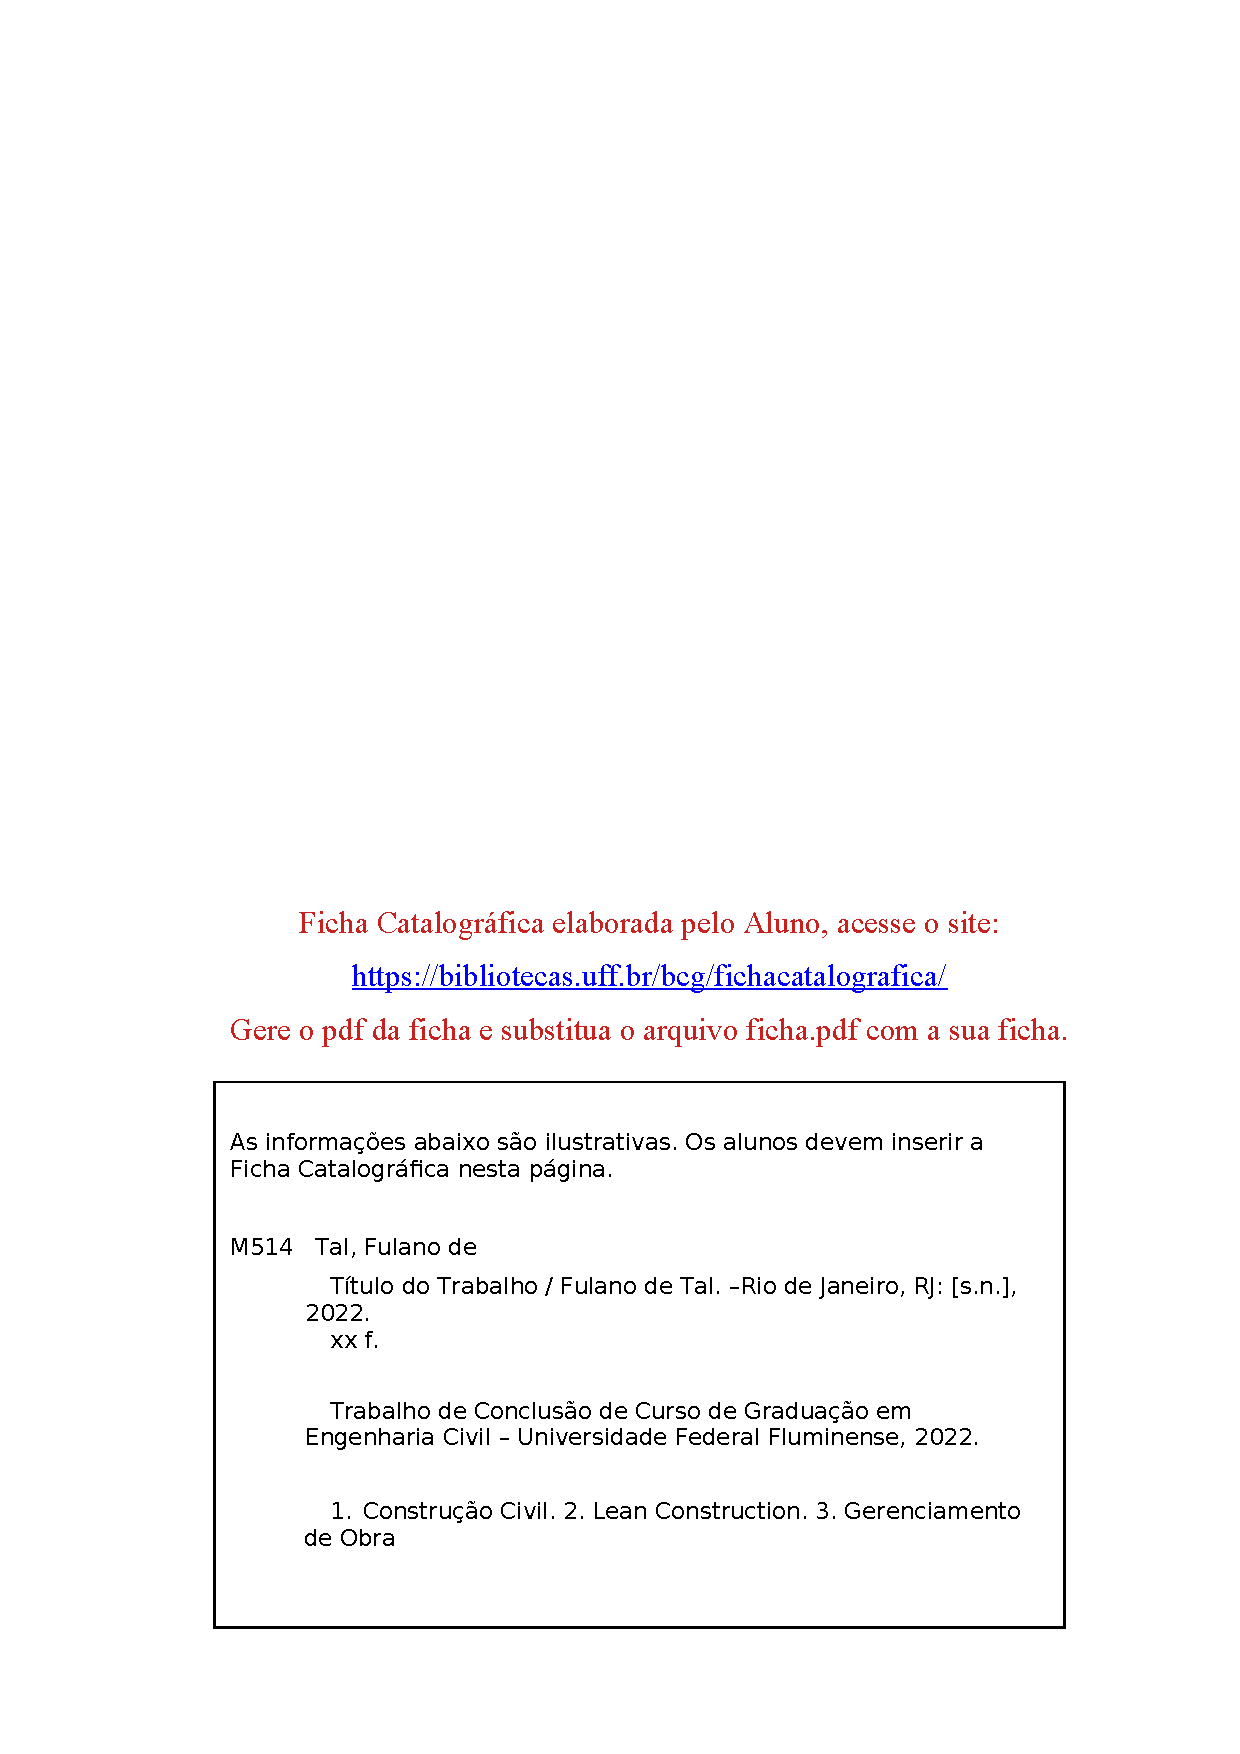
\includepdf[pages=-]{pretextuais/ficha.pdf}                                                                             % https://bibliotecas.uff.br/bcg/fichacatalografica/

% Folha de aprovação
\begin{folhadeaprovacao}

  \begin{center}
  \vspace*{-1.2cm}
    {\imprimirautor}

    \vspace*{\fill}
    {\textbf{\imprimirtitulo}}
    \vspace*{\fill}
    
    \hspace{.45\textwidth}
    \begin{minipage}{.5\textwidth}
        \imprimirpreambulo
    \end{minipage}%
    \vspace*{\fill}
   \end{center}
    
  \begin{flushleft}
  	 Aprovado em: \underline{\hspace{1.5cm}} de \underline{\hspace{4cm}} de \underline{\hspace{2cm}}
  \end{flushleft}
  \begin{center}
  \vspace*{2 cm}
  \textbf{BANCA EXAMINADORA}
   \assinatura{Prof. André da Costa Pinho, D.Sc. - UFF
   }
   \assinatura{Prof. Bruno Soares Moreira Cesar Borba, D.Sc. - UFF
   }
   \assinatura{Prof. Marcio Andre Ribeiro Guimaraens, D.Sc. - UFF
   }



\vspace*{\fill}

{\imprimirlocal}
\par
{\imprimirdata}
 \vspace*{-0.7cm}
 
 \end{center}
\end{folhadeaprovacao}

% Dedicatória
\begin{dedicatoria}
 \vspace*{\fill}
 \noindent
  \raggedleft
 \begin{minipage}{.54\textwidth}
   Em memória de minha querida avó Célia, por toda a sua paciência, carinho e amor incondicionais.
 \end{minipage}
\end{dedicatoria}


% Agradecimentos
\begin{agradecimentos}
\sloppy	

Agradeço aos meus pais, Débora e Gilvan, por sempre me apoiarem nas minhas escolhas, me ajudado a superar os obstáculos 
que surgiram no caminho e sempre estarem presentes nos momentos mais importantes. Obrigado por acreditarem em mim, por 
terem abdicado de tantas coisas para me proporcionar uma educação de qualidade e me ensinado a importância do esforço, 
estudo e trabalho. Serei eternamente grato pelos esforços e sacrifícios que fizeram por mim. Vocês sempre serão os meus 
maiores exemplos na vida.

À minha irmã, Letícia, por ser meu alívio cômico por todos esses anos. À minha família, por compreender minhas ausências
e por todos os aprendizados que me proporcionaram.

À minha companheira, Juliana, por ter me apoiado, incentivado e compreendido nos momentos de dificuldade. Por ter me 
ajudado a manter a calma e acreditar que eu era capaz de superar qualquer obstáculo. Obrigado por ser a
minha maior incentivadora e por nunca me deixar desistir nos momentos nos quais nem eu acreditava mais em mim.

Aos amigos que fiz durante a graduação, que sem dúvidas espero levar para a vida toda. Sem vocês o caminho teria sido
muito mais difícil. Agradeço por todos os momentos de descontração, pelas risadas, pelos estudos em grupo e, 
principalmente, pelo revezamento de faltas nas disciplinas mais chatas. À Faraday E-Racing, que representou um marco
na minha trajetória acadêmica e me proporcionou aprendizados e oportunidades essenciais para a minha formação.

Ao professor André Pinho, por, além de ter sido um dos melhores professores com quem já tive aula, ter me orientado 
durante o desenvolvimento deste trabalho de maneira exemplar. Agradeço também aos professores Flávio Martins, Felipe 
Sass e Marcio Guimaraens, por me lembrarem em cada aula do motivo pelo qual escolhi a Engenharia Elétrica. 

\end{agradecimentos}

% Epígrafe
%\begin{epigrafe}
    \vspace*{\fill}
	\begin{flushright}
		Não vos amoldeis às estruturas deste mundo, \\
		mas transformai-vos pela renovação da mente, \\
		a fim de distinguir qual é a vontade de Deus: \\
		o que é bom, o que Lhe é agradável, o que é perfeito.\\
		(Bíblia Sagrada, Romanos 12, 2)
	\end{flushright}
\end{epigrafe}

% Resumos
% resumo em português
\begin{resumo}
\noindent
A matriz elétrica brasileira é caracterizada por uma dependência significativa de fontes renováveis, especialmente a
geração hidrelétrica. Essa dependência torna o sistema elétrico vulnerável a variações climáticas, como secas 
prolongadas que podem ser intensificadas por fenômenos como o El Niño e La Niña, afetando a disponibilidade 
de água nos reservatórios e, consequentemente, a geração de energia. Com o crescimento da fonte eólica, também vulnerável a 
variações climáticas, é necessário investigar o impacto dessas variáveis na operação do Sistema Interligado Nacional 
(SIN), com ênfase nas fontes hidráulica, térmica e eólica. Este trabalho analisa séries históricas disponibilizadas pelo Operador Nacional 
do Sistema Elétrico (ONS) e variáveis que definem o fenômeno El Niño, obtidas do ERA5, para avaliar os efeitos desses fenômenos
na geração de energia elétrica. Modelos de regressão e aprendizado de máquina são aplicados para analisar
o impacto dessas variáveis na geração de energia.

\vspace{0.2cm}
\noindent
Palavras-chave: Geração de energia. Clima. Planejamento energético. Machine learning.
\end{resumo}

% resumo em inglês
\begin{resumo}[Abstract]	
\begin{otherlanguage*}{english}
\noindent 
\textit{The Brazilian electrical system is characterized by a significant dependence on renewable sources, especially hydropower generation. 
This dependence makes the electric system vulnerable to climatic variations, such as prolonged droughts and phenomena such as
El Niño (EN) and La Niña (LN), which can affect the availability of water in reservoirs and, consequently, energy generation. 
With the adoption of wind power, also vulnerable to climatic variations, it is necessary to investigate the impact of 
climatic variables on the operation of the National Interconnected System (SIN), with an emphasis on hydraulic, wind and 
thermal sources. This work analyzes historical series provided by the National Electric System Operator (ONS) and variables 
that define the El Niño phenomenon, obtained from the European Centre for Medium-Range Weather Forecasts (ECMWF) 
Reanalysis project (ERA5), to evaluate the effects of these phenomena on electricity generation. 
Regression and machine learning models are applied to analyze the impact of these variables on energy generation.}

\vspace{0.2cm}
\noindent
Key-words: Energy generation. Climate. Risk mitigation. Machine learning.
\end{otherlanguage*}
\end{resumo}

% Lista de ilustrações, tabelas e algoritmos
\renewcommand{\listfigurename}{}                                                                                        % Retira o nome da lista
\pretextualchapter{Lista de Figuras}                                                                                    % Capítulo sem numeração
\listoffigures*                                                                                                         % * indica que a lista não vai para o sumário
\cleardoublepage

\renewcommand{\listtablename}{}
\pretextualchapter{Lista de Tabelas}
\listoftables*
\cleardoublepage

\cleardoublepage

% Lista de abreviaturas e siglas
\begin{siglas}
  \item[ONS] Operador Nacional do Sistema Elétrico
  \item[EPE] Empresa de Pesquisa Energética
  \item[SIN] Sistema Interligado Nacional
  \item[] 
\end{siglas}

% Sumário
\renewcommand{\contentsname}{}	% Retira o nome da lista
\pretextualchapter{Sumário}
\tableofcontents*
\cleardoublepage

% Elementos textuais
% ----------------------------------------------------------------------------------------------------------------------
\textual

% Introdução
% Introdução e Trabalhos Relacionados (capítulos 1 e 2)
% ----------------------------------------------------------------------------------------------------------------------
\chapter{Introdução}
\sloppy																													% Para justificar o texto

\section{Contexto}
Historicamente, a matriz elétrica brasileira é considerada uma das mais limpas do mundo, com destaque para a fonte
hidráulica, que é responsável pela maior parte da geração de energia elétrica no país. Nos últimos anos, outras fontes
de geração vêm sendo incorporadas ao sistema, das quais destacam-se a eólica e solar fotovoltaica, conforme observado na
Figura \ref{fig:geracao_anual_por_fonte}, elaborada a partir de dados brutos de geração centralizada obtidos do Operador
Nacional do Sistema Elétrico (ONS), sem considerar a geração distribuída.

\begin{figure}[!ht]
	\IBGEtab{\caption{Geração centralizada anual por fonte}
			 \label{fig:geracao_anual_por_fonte}}
	{\includesvg[scale=1]{figuras/geracao_anual_percentual}}
	{\fonte{o autor, a partir de dados do ONS.}}
\end{figure}

Nota-se, em especial, um crescimento significativo da geração eólica, observado a partir de 2015, e uma diminuição 
significativa da contribuição de geração térmica média no panorama geral nos anos seguintes. Em 2023, a fonte eólica 
foi responsável por 48\% da expansão da capacidade instalada total de 10,19 GW \cite{EPE2024}. Essa expansão se dá em 
função do maior número de empreendimentos participantes nos Leilões de Energia Elétrica do Ambiente de Contratação 
Regulada (ACR) realizados pela Empresa de Pesquisa Energética (EPE). Isso ocorre, dentre outros fatores, devido à queda 
nos custos de aerogeradores e painéis fotovoltaicos, além do fator "combustível zero" dessas fontes, o que torna novos 
empreendimentos mais atrativos economicamente para os agentes.

Embora essa expansão seja positiva, poupando recursos hídricos, contribuindo para a diversificação da matriz elétrica e
reduzindo o acionamento de usinas térmicas, essas fontes possuem características intrínsecas que as tornam intermitentes,
como a incidência solar e a velocidade do vento. Sendo assim, uma alta dependência dessas fontes tem o potencial
de tornar o sistema como um todo mais vulnerável.

Além disso, ao analisar a curva de carga do SIN, observa-se que, embora o seu pico ocorra no início da 
tarde, momento no qual a geração solar fotovoltaica apresenta significativa contribuição, o período noturno também 
apresenta carga considerável, conforme a Figura \ref{fig:carga_max_dia}, que mostra a curva de carga do SIN para o 
dia 15 de março de 2024, dia em que registrou-se um recorde de demanda máxima instantânea de 102.478 MW, segundo o ONS.

\begin{figure}[!ht]
	\IBGEtab{\caption{Curva de carga diária do SIN em base horária}
			 \label{fig:carga_max_dia}}
	{\includesvg[scale=1]{figuras/carga_max_dia_2024-03-15}}
	{\fonte{o autor, a partir de dados do ONS.}}
\end{figure}

\section{Motivação}
Em um contexto no qual a implementação de sistemas de armazenamento de energia elétrica ainda é incipiente,
a matriz segue bastante dependente da fonte hidráulica e, de maneira complementar, das térmicas. A dependência da fonte
hidráulica, por sua vez, torna o sistema elétrico vulnerável a eventos climáticos extremos ocasionados pelas mudanças
climáticas. Por exemplo, em 2021, verificou-se um acionamento recorde de usinas térmicas e uma geração hidráulica 
percentual mínima. Isso se deve em razão da forte crise hídrica enfrentada pelo Brasil no período, a pior dos últimos 91 anos
até então. \cite{Soares2023}

\begin{figure}[!ht]
	\IBGEtab{\caption{Curva de carga do SIN em base mensal}
			 \label{fig:carga_anual}}
	{\includesvg[scale=1]{figuras/carga_anual}}
	{\fonte{o autor, a partir de dados do ONS.}}
\end{figure}

Portanto, o estudo do sistema elétrico brasileiro, no contexto de cenários de eventos
climatológicos extremos é altamente relevante para a segurança energética do país, considerando a tendência crescente
na curva de carga do SIN, ilustrada na Figura \ref{fig:carga_anual}, e uma projeção de crescimento médio anual de 3,2\%. \cite{pen2024}

Ao analisar a geração hidráulica bruta na Figura \ref{fig:geracao_hidraulica_bruta}, evidenciam-se pontos nos 
quais a geração é reduzida. Isso ocorre devido à sazonalidade das vazões nas bacias hidrográficas, responsáveis pelo 
abastecimento dos reservatórios. Considerando a amostragem em base mensal, observa-se que a geração é reduzida nos meses
de inverno, período caracterizado por menor ocorrência de precipitação e, consequentemente, menor vazão nos rios. Por
outro lado, nos meses de verão, a geração atinge seus maiores valores.

\begin{figure}[!ht]
	\IBGEtab{\caption{Geração hidráulica total em base mensal}
			 \label{fig:geracao_hidraulica_bruta}}
	{\includesvg[scale=1]{figuras/geracao_hidraulica_bruta}}
	{\fonte{o autor, a partir de dados do ONS.}}
\end{figure}

Esse comportamento é esperado, uma vez que a geração hidráulica é diretamente influenciada pelas condições
que afetam a vazão dos rios. No entanto, a ocorrência de eventos climáticos como o El Niño-Oscilação Sul (ENSO) pode
favorecer condições que impactam diretamente no potencial de geração hidráulica. \cite{de2012influencia}

\begin{figure}[!ht]
	\IBGEtab{\caption{Índice ONI (Oceanic Niño Index)}
			 \label{fig:oni}}
	{\includesvg[scale=1]{figuras/oni}}
	{\fonte{o autor, a partir de dados do ECMWF}}
\end{figure}

Fenômenos como o ENSO são monitoradas por meio de índices como o ONI (Oceanic Niño Index), que classifica os 
eventos em três categorias: \textit{El-Niño} (EN), \textit{La-Niña} (LN) e neutro. A Figura \ref{fig:oni} mostra a 
classificação dos eventos de EN e LN ocorridos entre 2000 e 2024, na qual a escala de cores indica a intensidade do 
evento, representado pela anomalia, que é a diferença do valor observado para um período em relação à sua média histórica.

Fundamentalmente, no sistema elétrico brasileiro, cuja fonte hidráulica constitui a base da matriz, é essencial, para um
planejamento energético eficiente, otimizar o sistema de modo a considerar a incerteza associada à disponibilidade de recursos
hidrológicos futuros. Dessa forma, estima-se o valor da geração hidrelétrica que poderia substituir a geração térmica a curto
ou longo prazo, de modo a reduzir os custos do sistema e o risco de utilizar reservatórios de maneira desnecessária, garantindo
assim o atendimento à demanda futura, principalmente em casos de escassez hídrica.

Com a introdução de fontes como a eólica, a incerteza referente aos perfis de velocidade do vento também deve ser considerada
para o planejamento energético. Os estudos de planejamento são realizados por meio de modelos computacionais como o NEWAVE, 
DECOMP e DESSEM, do Centro de Pesquisas de Energia Elétrica (CEPEL), que consideram diferentes horizontes temporais: longo, 
médio e curto prazos, respectivamente. Também há outras soluções disponíveis no mercado, como o PSR SDDP, que engloba todos
os horizontes temporais. Considerando o escopo deste trabalho, o modelo NEWAVE será brevemente apresentado no capítulo seguinte.

Embora esses modelos sejam amplamente utilizados pelo setor elétrico brasileiro, sendo consolidados como ferramentas
confiáveis e essenciais para o planejamento energético, eles não consideram variáveis externas, como fenômenos climáticos
como o EN e LN, que podem impactar a geração de energia elétrica. Esses modelos são baseados em dados históricos de
vazões e velocidade do vento, que são obtidos a partir de medições locais, além de dados individuais de cada usina.

\section{Objetivo}
Este trabalho tem como objetivo investigar o impacto de variáveis climáticas externas na geração 
de energia elétrica no Brasil, com foco nas fontes hidráulica, térmica e eólica. Para tanto, foram empregadas técnicas 
computacionais para relacionar as séries históricas de geração com as séries de variáveis 
climáticas, através de modelos lineares, não lineares e neurais. 

Além disso, foram utilizadas séries históricas de geração e carga disponibilizados pelo ONS, bem como séries históricas de variáveis 
climáticas de temperatura da superfície do mar, obtidas a partir de dados do ERA5, um projeto de reanálise atmosférica 
proposto por \citeonline{Hersbach2020}, que combina resultados de modelos computacionais com observações de diferentes fontes,
como satélites e estações meteorológicas, resultando em um \textit{dataset} global de alta resolução espacial e temporal.

A partir dessa investigação, espera-se poder avaliar o impacto dessas variáveis na geração de energia elétrica,
o que pode contribuir para o planejamento energético do país, especialmente em cenários de eventos climáticos extremos e
tendências climáticas.

É importante salientar que outras variáveis externas poderiam ser incorporadas ao estudo, ou até mesmo uma combinação entre
 variáveis locais e externas. Também poderiam ser considerados indicadores econômicos e outros dados relevantes. 
No entanto, este trabalho considera apenas as variáveis relacionadas ao fenômeno EN e LN, uma vez que estudos indicam
uma alta correlação entre esses fenômenos e o regime de chuvas no Brasil \cite{de2012influencia, Andreoli2016}, sendo a 
incorporação de outras variáveis reservada para trabalhos futuros.

% ----------------------------------------------------------------------------------------------------------------------
\section{Estrutura do Trabalho}
No capítulo 1, é feita uma breve introdução apresentando o contexto, motivação, objetivo e a estrutura do trabalho. Uma
breve análise da matriz elétrica é apresentada, com foco no histórico recente e no crescimento da geração eólica. Também
são apresentadas as curvas de carga do SIN e de geração hidráulica. Uma breve contextualização acerca dos fenômenos do
ENSO e a importância do modelo NEWAVE para o planejamento energético do país são apresentadas. Por fim, é apresentado
o objetivo do trabalho e a estrutura do documento. O capítulo 2 apresenta um panorama acerca de trabalhos relacionados ao tema.

No capítulo 2, a fundamentação teórica necessária para a compreensão do projeto é apresentada. São abordados os fatores
que fazem com que os fenômenos do EN e LN impactem o regime de chuvas no Brasil e a sua relação com a geração de 
energia elétrica. Também será feita uma breve introdução ao modelo NEWAVE,
que é amplamente utilizado pelo setor elétrico brasileiro para planejamento energético. Por fim, serão apresentados os modelos 
de previsão de séries temporais implementados, com foco no modelo neural, uma implementação baseada na arquitetura 
\textit{TSMixer} desenvolvida pela Google.

O capítulo 3 mostra a metodologia utilizada para a realização do projeto. Serão apresentados os conjuntos de dados
considerados e suas respectivas etapas de obtenção, tratamento e análise. Além disso, será apresentada a metodologia
utilizada para implementação dos modelos de previsão, incluindo seus parâmetros e métricas de avaliação.

O capítulo 4 apresenta os resultados do projeto. Para cada modelo, serão apresentados os resultados de previsão, métricas 
de avaliação e uma análise crítica dos resultados obtidos. No capítulo 5, serão apresentadas as considerações finais.

% Fundamentação Teórica
% Apresentar estudos que contemple a temática abordada. Respeitar a autoria,
% nas citações diretas e indiretas. Evitar parágrafos muito longos. Evitar seções e
% subseções muito curtas.

\chapter{Fundamentação Teórica}
\section{Impacto do ENSO na Geração de Energia Elétrica}
O ENSO é um fenômeno que ocorre no Oceano Pacífico Equatorial, caracterizado por variações na temperatura da superfície
do mar (TSM) em regiões específicas, como ilustrado na Figura \ref{fig:regioes_enso}. Segundo \citeonline{Andreoli2016}, o 
fenômeno é um dos principais fatores que influenciam os padrões de vento e precipitação em diversas regiões da América 
do Sul e seus efeitos se estendem por todas as regiões do Brasil.

De acordo com \citeonline{Capozzoli2017}, diferentes fases do ENSO resultam em padrões distintos de precipitação sobre
o território brasileiro, variando de acordo com a região e a estação do ano. Sendo assim, há um impacto direto sobre a 
disponibilidade de recursos hídricos para a geração hidrelétrica.

A região Sul é uma das mais consistentemente afetadas. Eventos de El Niño tendem a causar precipitação acima da média,
particularmente durante a primavera e o verão, enquanto eventos de La Niña estão associados à condições de seca.

A região Sudeste apresenta uma resposta mais complexa, sendo consdierada uma zona de transição. A bacia do Rio Paraná,
em especial, apresenta sensibilidade aos fenômenos do ENSO, tendo apresentado tendência de aumento de vazão durante alguns
eventos de El Niño.

Para as regiões Norte e Nordeste, eventos de El Niño estão associados a períodos de seca, enquanto eventos de
La Niña tendem a trazer chuvas acima da média. No entanto, é importante destacar que outros fenômenos atmosféricos podem
interferir com esses padrões, modulando os efeitos do ENSO.

Sendo assim, verifica-se que as variações induzidas pelos fenômenos do ENSO traduzem-se diretamente em variações nas
vazões dos rios que alimentam as bacias, que por sua vez impactam diretamente o potencial de geração da fonte hidráulica.

\begin{figure}[!ht]
	\IBGEtab{\caption{Regiões do fenômeno El Niño-Oscilação Sul (ENSO)}
			 \label{fig:regioes_enso}}
	{\includesvg[scale=1]{figuras/regioes_enso_global}}
	{\fonte{o autor.}}
\end{figure}

\section{O Modelo NEWAVE}
\label{sec:newave}

Desenvolvido e mantido pelo Centro de Pesquisas de Energia Elétrica (CEPEL) e amplamente utilizado pelo setor elétrico 
brasileiro para definição de estratégias e tomada de decisão, o NEWAVE é um modelo de otimização que busca minimizar os 
custos de operação do sistema, considerando a incerteza das afluências futuras e a operação de um sistema 
hidro-térmico-eólico interligado. O modelo é utilizado para estudos como:
\begin{itemize}
	\item Elaboração do Plano Decenal de Expansão de Energia (PDE), pela EPE;
	\item Elaboração do Programa Mensal de Operação (PMO) e Plano de Operação Energética (PEN), pelo ONS;
	\item Formação de preços, como no cálculo do Preço de Liquidação das Diferenças (PLD) pelo CCEE;
	\item Cálculo de Garantia Física e da Energia Assegurada para empreendimentos de geração participantes nos leilões 
    de energia elétrica, pela EPE;
	\item Elaboração de diretrizes para os leilões de energia, pela EPE.
\end{itemize}

Em resumo, o modelo emprega a Programação Dinâmica Dual Estocástica (PDDE), uma técnica de otimização que permite lidar 
com as incertezas ligadas às afluências futuras sem que o modelo se torne computacionalmente impraticável, considerando 
múltiplos reservatórios, interconexões e o horizonte temporal de médio e longo prazos.

\subsection{Representação das Usinas}
O NEWAVE modela o sistema de geração hidrelétrico em Reservatórios Equivalentes de Energia (REEs), que são grupos de
usinas associadas a um subsistema ou submercado de energia. Cada subsistema pode conter mais de um REE, possibilitando
diferenciar bacias hidrográficas com regimes distintos, ainda que pertençam a um mesmo subsistema. 

Além disso, cada REE é definido por um conjunto de parâmetros que são calculados a partir das características indivuduais 
de cada usina. Nas versões mais recentes do modelo, também é possível considerar todas as usinas indivudalmente ou operar
de maneira híbrtida, ou seja, considerando alguns REEs e outras usinas individualmente.

As usinas termelétricas são representadas no modelo através de classes térmicas. Cada classe agrupa usinas com custos 
semelhantes e está associada a um subsistema. Cada classe também é definida por um conjunto de parâmetros calculados
a partir das características individuais de cada usina.

Nas versões mais recentes do modelo, a fonte eólica também é modelada. De maneira similar, os parques eólicos são agrupados
em Parques Eólicos Equivalentes (PEE). O agrupamento é feito a aprtir de dados de cadastro de cada prque eólico, estado,
submercado, função de produção (curva relacionando a velocidade do vento com a potência gerada), dados sobre torres de
medição e séries históricas de velocidade do vento.

\subsection{Dados de Entrada}
O modelo requer um conjunto de dados de entrada que inclui as características das usinas, dados dos subsistemas, demanda,
séries históricas de vazões e ventos, cronogramas de expansão, restrições operativas, dentre outros. Observa-se, portanto, 
que todos os dados de entrada são locais e, portanto, o modelo não considera variáveis externas, como fenomênos climáticos
como o EN e LN, que podem impactar a geração de energia elétrica. 

Ainda que as últimas versões do modelo apresentem campos previstos para a entrada de dados do ENSO, esses campos
estão marcados como "não implementados". Dessa forma, entende-se que o modelo não considera diretamente o impacto 
dessas variáveis. No entanto, vale destacar que essas variáveis externas podem ser utilizadas para elaborar as séries históricas de 
vazões e velocidade de ventos utilizadas como dados de entrada. 

\section{Modelos Linear e Não-linear}
fazer uma introdução sobre os modelos lineares e não lineares...

\subsection{Modelo Linear}

\subsection{Modelos Não-lineares: Random Forest e Gradient Boosting}

\section{Modelo Neural}
Atualmente, os modelos neurais mais avançados utilizam a arquitetura \textit{Transformer}, que são modelos neurais com um
mecanismo de atenção que permite ao modelo focar em diferentes partes da entrada de dados ao processar informações. Essa
arquitetura foi introduzida no artigo \textit{"Attention is All You Need"} de \citeonline{Vaswani2017} e hoje é a arquitetura
por trás dos principais \textit{Large Language Models} (LLMs) comercialmente disponíveis.

Inicialmente concebido para tarefas de tradução, modelos baseados nessa arquitetura demonstraram resultados superiores
em outras aplicações e hoje são amplamente utilizados em diversas áreas, incluindo previsão de séries temporais. No entanto,
esses modelos são altamente complexos e exigem um alto poder computacional para treinamento e inferência.

Além disso, conforme demonstrado por \citeonline{Zeng2022}, modelos baseados em \textit{Transformers} podem produzir
resultados inferiores quando comparados a modelos mais simples. 

Dessa forma, uma abordagem alternativa foi proposta por \citeonline{Chen2023}, uma arquitetura mais simples em comparação
aos \textit{Transformers}, mas com resultados bastante superiores

% Desenvolvimento
\chapter{Metodologia}
\section{Abordagem computacional}

O projeto tem como objetivo analisar o impacto de variáveis climatológicas, como anomalias e outros índices, na geração
de energia elétrica no Brasil. Para isso, foram adotadas técnicas computacionais para processamento de séries temporais,
correlação de variáveis, \textit{feature selection}, análise de componentes principais e implementação de modelos de 
regressão e aprendizado de máquina. 

As etapas de processamento intensivo foram otimizadas para execução em paralelo,
de modo a melhor utilizar os recursos computacionais. Todo o processamento foi realizado em um computador com 
processador AMD Ryzen 5900X e 32 GB de memória RAM, utilizando todas as 24 \textit{threads} disponíveis.

\begin{table}[htb]
  \centering
   \IBGEtab{
    \caption{Bibliotecas utilizadas no projeto}
    \label{tab:bibliotecas}
    }{
    \begin{tabular}{llll}
  		  \hline
    	  \textbf{Biblioteca} & \textbf{Descrição} & \textbf{Versão} \\ \hline
        numpy & Cálculos numéricos e manipulação de arrays & 1.26.4 \\
        pandas & Manipulação e análise de dados (DataFrames) & 2.2.3 \\
        requests & Requisições HTTP & 2.32.3 \\
        urllib3 & Gerenciamento de conexões HTTP & 2.2.3 \\
        alive\_progress & Barra de progresso para loops & 3.2.0 \\
        netCDF4 & Leitura de arquivos NetCDF & 1.7.2 \\
        cdsapi & API para download de dados do ECMWF & 0.7.5 \\
        geopandas & Manipulação de dados geoespaciais & 1.0.1 \\
        matplotlib & Visualização de dados & 3.9.2 \\
        scikit-learn & Ferramentas de aprendizado de máquina & 1.5.2 \\
        scipy & Ferramentas e algoritmos matemáticos & 1.14.1 \\
        \hline
    \end{tabular}
    }{
      \fonte{o autor.}}
\end{table}

Além disso, toda a base de código foi desenvolvida em Python versão 3.12 e está disponível em um repositório público no
GitHub. O projeto foi organizado em módulos, cada um responsável por uma etapa do processo, desde a obtenção dos dados 
até a implementação dos modelos de aprendizado de máquina. A tabela \ref{tab:bibliotecas} mostra as bibliotecas 
utilizadas no projeto.

\section{Obtenção e pré-processamento dos dados}
\subsection{Séries históricas do ONS}

A primeira etapa do projeto consiste na consolidação das séries históricas de geração, carga e variáveis hidrológicas,
que são disponibilizadas publicamente no portal Dados Abertos do ONS, a partir do ano 2000. As séries referentes 
às variáveis hidrológicas são disponibilizadas em base diária, e os dados de geração e carga são disponibilizados em 
base horária. Sendo assim, a fim de obter uma amostragem representativa e suficiente para aplicação dos modelos 
computacionais, optou-se por utilizar a base temporal diária. 

Os dados de geração são disponibilizados em Mega Watt médio (MWmed) por fonte de energia, subsistema, estado, 
modalidade de operação, entre outras variáveis. Os dados de carga também são disponibilizados em MWmed e contêm 
informações sobre a carga em cada subsistema do SIN.

Para as séries de geração, os dados de 2000 a 2021 são agrupados pelos respectivos anos, e a partir de 2022,
as informações estão agrupadas em arquivos por mês e ano. Para as séries de carga, os dados são disponibilizados por
ano. Como o ONS não disponibiliza Aplication Programming Interface (API) para a obtenção dos dados diretamente, foi 
necessário uma outra abordagem, a fim de evitar o download manual dos dados. 

Após identificar o padrão de nomenclatura utilizado pelo ONS para os arquivos, foram desenvolvidas as funções 
\textit{GetGeracao}, \textit{GetCarga} e \textit{GetVazao} para obtenção dos dados de geração, carga e hidrológicos,
respectivamente. Os arquivos foram baixados por meio de requisições HTTP, utilizando a biblioteca \textit{requests} e
a biblioteca \textit{urllib3} para gerenciar as conexões. Além disso, as funções realizam o download dos arquivos em
paralelo, utilizando todas as threads disponíveis do sistema. Ao todo, cerca de 10 GB de dados em arquivos Comma 
Separated Values (CSV) foram consolidados.


\begin{algorithm}
\caption{Pseudocódigo para download dos dados de geração}
\label{alg:get_geracao_pseudo}
\begin{algorithmic}[1]
  \Function{GetGeracao}{anos, baseUrl}
    \State Inicializar barra de progresso para \textit{anos}
    \State Criar um executor de threads
    \State Submeter tarefas \Call{DownloadAno}{ano} para cada \textit{ano} em \textit{anos} ao executor
    \For{cada futuro \textit{f} retornado pelo executor}
      \State Aguardar resultado de \textit{f}
      \State Atualizar barra de progresso
    \EndFor
  \EndFunction
  \State
  \Function{DownloadAno}{ano}
    \If{ano < 2022}
      \State Construir URL: baseUrl + "GERACAO\_USINA-2\_{ano}.csv"
      \State Fazer requisição HTTP GET para a URL
      \If{Requisição bem-sucedida (status 200)}
        \State Abrir arquivo local "GERACAO\_USINA-2\_{ano}.csv" para escrita
        \For{cada bloco de dados recebido na resposta}
          \State Escrever bloco no arquivo local
        \EndFor
        \State Fechar arquivo local
        \State \Return Verdadeiro
      \Else
        \State \Return Falso
      \EndIf
    \Else
      \State Definir \textit{concluido} como Falso
      \For{cada \textit{mes} de 1 a 12}
        \State Formatar \textit{mes} com zero à esquerda se necessário
        \State Construir URL: baseUrl + "GERACAO\_USINA-2\_{ano}\_{mes}.csv"
        \State Fazer requisição HTTP GET para a URL
        \If{Requisição bem-sucedida (status 200)}
          \State Abrir arquivo local "GERACAO\_USINA-2\_{ano}\_{mes}.csv" para escrita
          \For{cada bloco de dados recebido na resposta}
            \State Escrever bloco no arquivo local
          \EndFor
          \State Fechar arquivo local
          \State Definir \textit{concluido} como Verdadeiro
        \Else
          \State Definir \textit{concluido} como Falso
        \EndIf
      \EndFor
      \State \Return \textit{concluido}
    \EndIf
  \EndFunction

\end{algorithmic}
\end{algorithm}


Considerando o período de 2000 a 2024, foram consolidados ao todo 9132 amostras diárias para cada variável. Caso fosse
considerada a amostragem mensal, o número de amostras seria de apenas 300, o que poderia não ser suficiente para
a aplicação dos modelos. Ainda assim, análises em base mensal poderão ser realizadas posteriormente, considerando a
possibilidade de transofrmação dos dados para essa escala temporal.

Toda a manipulação dos dados foi realizada utilizando a biblioteca \textit{pandas}, de modo a facilitar a seleção das
variáveis de interesse

\begin{table}[htb]
  \centering
   \IBGEtab{
    \caption{Parâmetros dos dados de geração}
    \label{tab:geracao}
    }{
      \begin{tabular}{llll}
          \hline
          \textbf{Parâmetro} & \textbf{Descrição} & \textbf{Tipo} \\ \hline
          din\_instante & Instante de aferição & Datetime\\
          nom\_subsistema & Subsistema da usina & String\\
          id\_estado & Estado onde a usina está localizada & String\\ 
          nom\_tipousina & Tipo de usina & String\\
          nom\_tipocombustivel & Tipo de combustível & String\\
          nom\_usina & Nome da usina & String\\
          val\_geracao & Geração de energia (MWmed) & Float\\ \hline
      \end{tabular}
    } {
      \fonte{\citeonline{pen2024}}
      \nota{Variáveis não utilizadas foram omitidas.}
    }
\end{table}

\begin{table}[htb]
  \centering
   \IBGEtab{
    \caption{Parâmetros dos dados de carga}
    \label{tab:carga}
    }{
    \begin{tabular}{llll}
  		  \hline
    	  \textbf{Parâmetro} & \textbf{Descrição} & \textbf{Tipo} \\ \hline
        din\_instante & Instante de aferição & Datetime\\
        nom\_subsistema & Subsistema da usina & String\\
        val\_cargaenergiahomwmed & Carga de energia (MWmed) & Float\\ \hline
    \end{tabular}
    }{
      \fonte{\citeonline{pen2024}}}
\end{table}

Verifica-se, a partir da tabela \ref{tab:geracao}, que os dados de geração contém informações que permitem uma análise 
detalhada da operação do SIN em diferentes níveis de granulidade. Dessa maneira, possíveis impactos em diferentes 
escalas geográficas e temporais poderão ser avaliados. Por outro lado, a tabela \ref{tab:carga} mostra que os dados de
carga não possuem a mesma granulidade que os dados de geração, limitando a análise a nível de subsistema, conforme a
figura \ref{fig:subsistemas_brasil}.

\begin{figure}[!ht]
	\IBGEtab{\caption{Subsistemas do SIN}
			 \label{fig:subsistemas_brasil}}
	{\includesvg[scale=1]{figuras/subsistemas_brasil}}
	{\fonte{o autor.}}
\end{figure}

\subsection{Séries históricas de variáveis climatológicas}
A fim de maximizar o potencial de análise do projeto, é essencial considerar um grande número de dados climatológicos, 
como anomalis de temperatura, precipitação, pressão, radiação solar, entre outros. Para isso, foram utilizados dados 
disponibilizados pelo ECMWF, NOAA e também do departamento de ciências atmosféricas da UNIFEI.

Os dados do ECMWF foram obtidos através da API do CDS (Climate Data Store), que permite o download de dados 
meteorológicos de alta resolução, sendo possível especificar a escala temporal e a área de interesse, especificando as 
coordenadas geográficas. Os dados do NOAA e UNIFEI foram obtidos através de requisições HTTP.

É importante ressaltar que, embora a maioria dos dados climatológicos seja disponibilizada em base mensal, alguns
possuem escala temporal diária, como alguns dados do ECMWF. Considerando que os dados de energia são disponibilizados em
base horária, diferentes análises poderão ser realizadas, considerando as escalas temporais diária e mensal. Para isso,
durante a etapa de pré-processamento dos dados, será realizada a consolidação dos dados de geração e carga de modo que
estejam na mesma escala temporal dos dados climatológicos.

Além disso, nas próximas etapas do projeto, será realizado a seleção das variáveis climatológicas mais relevantes para
a análise, considerando a correlação com a geração de energia. Para isso, serão utilizadas técnicas de \textit{feature
selection} e redução de dimensionalidade, como a análise de componentes principais. A tabela \ref{tab:variaveis_clima}
mostra as variáveis climatológicas utilizadas no projeto.

\subsection{Pré-processamento dos dados}


\section{Análise exploratória dos dados}


\section{Implementação dos modelos de regressão}


\subsection{Feature selection}


\subsection{Análise de componentes principais}


\subsection{Avaliação dos modelos de regressão}


\section{Implementação dos modelos de aprendizado de máquina}


\subsection{Feature selection}


\subsection{Análise de componentes principais}


\subsection{Avaliação dos modelos de aprendizado de máquina}


% Resultados
\chapter{Resultados}
Este capítulo apresenta os resultados obtidos na estimação da geração das fontes hidráulica, eólica e térmica. A análise 
se inicia com modelos de regressão linear e não linear (Random Forest) para estabelecer um baseline de performance e 
avaliar a linearidade das relações (Seções 5.1 e 5.2). Em seguida, na Seção 5.3, avalia-se o desempenho do modelo 
neural (\textit{Tiny Time Mixer}) em sua aplicação direta. Por fim, na Seção 5.3.2, demonstra-se o impacto e a 
eficácia do ajuste fino (\textit{finetuning}) deste modelo com a inclusão de variáveis do fenômeno ENSO, quantificando o ganho de 
acurácia obtido com a especialização do modelo. Serão apresentados os gráficos de geração total das fontes. Demais gráficos 
dos resultados para os subsistemas estão disponíveis no Apêndice B.

\section{Modelo Linear}
\subsection{Fonte Hidráulica}
A Figura \ref{fig:linear_hidraulica} apresenta os resultados da regressão linear para a fonte hidráulica. Para esse caso,
foram consdierados os dados de 2010 em diante. O conjunto de treino foi constituído pelos dados de 2010 a 2021, e o 
conjunto de teste pelos dados restantes. 

\begin{figure}[!ht]
  \IBGEtab{\caption{Regressão linear para fonte hidráulica (carga + ENSO) em base diária}
       \label{fig:linear_hidraulica}}
  {\includesvg[scale=.9]{figuras/linear_Hidráulica}}
  {\fonte{o autor.}}
\end{figure}
Fica evidente que, para a geração hidráulcia total, o modelo é capaz de estimar os valores de geração do conjunto de teste
com um valor de R² de 0,593, o que indica uma correlação moderada entre os valores estimados e os valores reais, considerando
as limitações do modelo linear. 

Para verificar a utilidade dos dados do ENSO, uma nova regressão foi realizada, dessa vez
considerando apenas a carga como variável independente, conforme a Figura \ref{fig:linear_hidraulica_carga}. Observa-se 
uma queda no valor de R² de 0,593 para 0,525, uma redução de 11,5\% na capacidade explicativa do modelo, indicando que a 
inclusão do ENSO melhora significativamente a predição. Além disso, o resultado é compatível com a fundamentação teórica 
apresentada no Capítulo 3, na qual a influência do ENSO na geração hidráulica é direta e significativa.

\begin{figure}[!ht]
  \IBGEtab{\caption{Regressão linear para fonte hidráulica (apenas carga) em base diária}
       \label{fig:linear_hidraulica_carga}}
  {\includesvg[scale=.9]{figuras/linear_Hidráulica_CARGA}}
  {\fonte{o autor.}}
\end{figure}

Embora o modelo linear atinja um R² de 0,593, o gráfico de dispersão (à esquerda) mostra que os pontos se 
afastam da linha ideal especialmente nos extremos. Nota-se que o modelo tende a subestimar os picos de geração 
(pontos acima da linha) e a superestimar os vales (pontos abaixo da linha), uma limitação característica da regressão 
linear ao tentar capturar a amplitude total de uma série com forte sazonalidade.

A fim de melhor avaliar os resultados, os demais gráficos serão apresentados em base temporal mensal, indicando a média 
dos valores de geração para cada mês em MWmed, consdierando os valores médios das variáveis independentes para o mesmo período. 
A Figura \ref{fig:linear_hidraulica_mensal} apresenta os resultados mensais da regressão linear para a fonte hidráulica, 
considerando a carga e o ENSO. 

\begin{figure}[!ht]
  \IBGEtab{\caption{Regressão linear para fonte hidráulica (carga + ENSO) em base mensal}
       \label{fig:linear_hidraulica_mensal}}
  {\includesvg[scale=.9]{figuras/linear_Hidráulica_mensal}}
  {\fonte{o autor.}}
\end{figure}
\begin{figure}[!ht]
  \IBGEtab{\caption{Regressão linear para fonte hidráulica (apenas carga) em base mensal}
       \label{fig:linear_hidraulica_mensal_carga}}
  {\includesvg[scale=.9]{figuras/linear_Hidráulica_mensal_CARGA}}
  {\fonte{o autor.}}
\end{figure}

Novamente, é realizado uma avaliação do modelo considerando apenas a carga, conforme a Figura 
\ref{fig:linear_hidraulica_mensal_carga}. Observa-se que, para a regressão mensal, a queda na performance do modelo é ainda
maior: o valor de R² cai de 0,519 para 0,420. Isso pode indicar que a inclusão de variáveis do ENSO é ainda mais significante 
para a base temporal mensal.

\subsection{Fonte Eólica e Térmica}
As Figuras \ref{fig:linear_eolica_mensal} e \ref{fig:linear_termica_mensal} apresentam os resultados para as fontes eólica 
e térmica, nos quais pode-se observar que o modelo não foi capaz de apresentar resultados satisfatórios, sugerindo
que a relação entre as variáveis independentes e dependentes pode ser não linear, validando a hipótese levantada nos capítulos
anteriores.

\begin{figure}[!ht]
  \IBGEtab{\caption{Regressão linear para fonte eólica (carga + ENSO) em base mensal}
       \label{fig:linear_eolica_mensal}}
  {\includesvg[scale=.9]{figuras/linear_Eólica_mensal}}
  {\fonte{o autor.}}
\end{figure}
\begin{figure}[!ht]
  \IBGEtab{\caption{Regressão linear para fonte térmica (carga + ENSO) em base mensal}
       \label{fig:linear_termica_mensal}}
  {\includesvg[scale=.9]{figuras/linear_Térmica_mensal}}
  {\fonte{o autor.}}
\end{figure}

A regressão para a fonte eólica resultou em um valor de R² de 0,004, o que indica que o modelo não é capaz de explicar a 
variabilidade dos dados, enquanto que para a fonte térmica, o valor de R² foi negativo, indicando que o modelo é pior do 
que uma média simples dos dados. Esses resultados corroboram a hipótese de que a relação entre as variáveis independentes 
e dependentes é não linear, o que justifica a escolha de modelos mais complexos para essas fontes.


\section{Modelo Não Linear}
\subsection{Fonte Hidráulica}
\begin{figure}[!ht]
  \IBGEtab{\caption{Random forest para fonte hidráulica}
       \label{fig:rf_hidraulica}}
  {\includesvg[scale=.9]{figuras/nlinear/rf_Hidráulica}}
  {\fonte{o autor.}}
\end{figure}
A Figura \ref{fig:rf_hidraulica} apresenta os resultados do modelo não linear para a fonte hidráulica, considerando os dados 
de carga e ENSO como variáveis independentes. O dataset utilizado contém dados a partir de 2010. Os resultados são
ligeiramente superiores aos do modelo de regressão linear, com um valor de R² de 0,525.

\subsection{Fonte Eólica e Térmica}
\begin{figure}[!ht]
  \IBGEtab{\caption{Random forest para fonte eólica}
       \label{fig:rf_eolica}}
  {\includesvg[scale=.9]{figuras/nlinear/rf_Eólica}}
  {\fonte{o autor.}}
\end{figure}
\begin{figure}[!ht]
  \IBGEtab{\caption{Random forest para fonte térmica}
       \label{fig:rf_termica}}
  {\includesvg[scale=.9]{figuras/nlinear/rf_Térmica}}
  {\fonte{o autor.}}
\end{figure}

As Figuras \ref{fig:rf_eolica} e \ref{fig:rf_termica} apresentam os resultados do modelo não linear para as fontes eólica 
e térmica, respectivamente. De maneira similar ao modelo linear, o modelo não linear também não é capaz de produzir resultados
satisfatórios para essas fontes.

Ainda que o modelo Random Forest apresente uma capacidade superior para modelar não-linearidades, os resultados para as 
fontes eólica e térmica permaneceram insatisfatórios. Essa dificuldade sugere que as relações temporais são complexas e 
podem ser mais bem capturadas por modelos como o avaliado a seguir.

\section{Modelo Neural}
\subsection{Modelo Pré-treinado}
Ao fazer a implementação \textit{oneshot}, todos os pesos do \textit{backbone}, as camadas escondidas, permanecem inalterados
em relação ao modelo pré treinado, e apenas a \textit{head}, ou cabeça de previsão, é ajustada para gerar a saída desejada,
considerando o número de variáveis dependentes.

A seguir serão apresentados os resultados da previsão \textit{oneshot} para cada fonte de geração, considerando os dados de carga e ENSO
como variáveis independentes. Para cada fonte, serão apresentados os resultados considerando as janelas de contexto e previsão
de 90/30 semanas e 512/96 dias. Demais gráficos dos resultados para os subsistemas estão disponíveis no Apêndice B.

\subsubsection{Fonte Hidráulica}
\begin{figure}[!ht]
  \IBGEtab{\caption{Oneshot para fonte hidráulica (contexto/previsão: 90/30 semanas)}
       \label{fig:oneshot_hidraulica_w90-30}}
  {\includesvg[scale=.9]{figuras/oneshot/os_Hidráulica_W90-30}}
  {\fonte{o autor.}}
\end{figure}
\begin{figure}[!ht]
  \IBGEtab{\caption{Oneshot para fonte hidráulica (contexto/previsão: 512/96 dias)}
       \label{fig:oneshot_hidraulica_d512-96}}
  {\includesvg[scale=.9]{figuras/oneshot/os_Hidráulica_D512-96}}
  {\fonte{o autor.}}
\end{figure}
As Figuras \ref{fig:oneshot_hidraulica_w90-30} e \ref{fig:oneshot_hidraulica_d512-96} apresentam os resultados da previsão
\textit{oneshot} para a fonte hidráulica, considerando as janelas de contexto e previsão de 90/30 semanas e 512/96 dias, respectivamente.
Observa-se que as métricas de avaliação foram superiores para o caso de 512/96 dias. Isso pode ser explicado devido à
taxa de amostragem diária, que permite uma maior quantidade de dados para o treinamento do modelo e maior número de 
janelas de contexto e previsão.

Para o caso de 90/30 semanas, o valor de R² foi de 0,573, enquanto que para o caso de 512/96 dias, o valor de R² foi de 0,581.
Esses valores são razoáveis, considerando a implementação \textit{oneshot}, sem ajuste fino para o dataset. Além disso, os
resultados são comparáveis aos resultados do modelo linear, o que sugere que a relação da geração hidráulica com as variáveis 
consideradas pode ser mais linear do que as demais fontes de geração.

\subsubsection{Fonte Eólica}
\begin{figure}[!ht]
  \IBGEtab{\caption{Oneshot para fonte eólica (contexto/previsão: 90/30 semanas)}
       \label{fig:oneshot_eolica_w90-30}}
  {\includesvg[scale=.9]{figuras/oneshot/os_Eólica_W90-30}}
  {\fonte{o autor.}}
\end{figure}
\begin{figure}[!ht]
  \IBGEtab{\caption{Oneshot para fonte eólica (contexto/previsão: 512/96 dias)}
       \label{fig:oneshot_eolica_d512-96}}
  {\includesvg[scale=.9]{figuras/oneshot/os_Eólica_D512-96}}
  {\fonte{o autor.}}
\end{figure}
As Figuras \ref{fig:oneshot_eolica_w90-30} e \ref{fig:oneshot_eolica_d512-96} apresentam os resultados da previsão
\textit{oneshot} para a fonte eólica, considerando as janelas de contexto e previsão de 90/30 semanas e 512/96 dias, respectivamente.
Observa-se que, para o caso de 90/30 semanas, o valor de R² foi de 0,683, enquanto que para o caso de 512/96 dias, o valor de R² foi de 0,826.

Esses valores são superiores aos resultados da fonte hidráulica, sugerindo que o modelo consegue capturar melhor a relação
entre as variáveis. Além disso, as métricas de avaliação foram consideravelmente superiores em comparação com os modelos
linear e não linear, sugerindo que, de fato, a relação entre as variáveis é extremamente não linear.

\subsubsection{Fonte Térmica}
\begin{figure}[!ht]
  \IBGEtab{\caption{Oneshot para fonte térmica (contexto/previsão: 90/30 semanas)}
       \label{fig:oneshot_termica_w90-30}}
  {\includesvg[scale=.9]{figuras/oneshot/os_Térmica_W90-30}}
  {\fonte{o autor.}}
\end{figure}
\begin{figure}[!ht]
  \IBGEtab{\caption{Oneshot para fonte térmica (contexto/previsão: 512/96 dias)}
       \label{fig:oneshot_termica_d512-96}}
  {\includesvg[scale=.9]{figuras/oneshot/os_Térmica_D512-96}}
  {\fonte{o autor.}}
\end{figure}
As Figuras \ref{fig:oneshot_termica_w90-30} e \ref{fig:oneshot_termica_d512-96} apresentam os resultados da previsão
\textit{oneshot} para a fonte térmica, considerando as janelas de contexto e previsão de 90/30 semanas e 512/96 dias, respectivamente.
A geração térmica apresentou o pior resultado entre as fontes, com um valor de R² de 0,183 para o caso de 90/30 semanas
e 0,531 para o caso de 512/96 dias. Ainda assim, os valores são consideravelmente superiores em comparação com os os
modelos linear e não linear.

\subsection{Impacto e Análise do Ajuste Fino}
\subsubsection{Fonte Hidráulica}
\begin{figure}[!ht]
  \IBGEtab{\caption{Finetune para fonte hidráulica (contexto/previsão: 90/30 semanas)}
       \label{fig:finetune_hidraulica_w90-30}}
  {\includesvg[scale=.9]{figuras/finetune/fn_Hidráulica_W90-30}}
  {\fonte{o autor.}}
\end{figure}
\begin{figure}[!ht]
  \IBGEtab{\caption{Finetune para fonte hidráulica (contexto/previsão: 512/96 dias)}
       \label{fig:finetune_hidraulica_d512-96}}
  {\includesvg[scale=.9]{figuras/finetune/fn_Hidráulica_D512-96}}
  {\fonte{o autor.}}
\end{figure}
As Figuras \ref{fig:finetune_hidraulica_w90-30} e \ref{fig:finetune_hidraulica_d512-96} apresentam os resultados do ajuste fino
para a fonte hidráulica, considerando as janelas de contexto e previsão de 90/30 semanas e 512/96 dias, respectivamente.

Observa-se que o ajuste fino melhorou em 4,53\% o valor de R² para o caso de 90/30 semanas, passando de 0,573 para 0,599.
Para o caso de 512/96 dias, o ajuste fino melhorou em 15,49\% o valor de R², passando de 0,581 para 0,671. Os resultados 
indicam que o processo de ajuste dos pesos do modelo é eficaz em melhorar a performance do modelo.

\subsubsection{Fonte Eólica}
\begin{figure}[!ht]
  \IBGEtab{\caption{Finetune para fonte eólica (contexto/previsão: 90/30 semanas)}
       \label{fig:finetune_eolica_w90-30}}
  {\includesvg[scale=.9]{figuras/finetune/fn_Eólica_W90-30}}
  {\fonte{o autor.}}
\end{figure}
\begin{figure}[!ht]
  \IBGEtab{\caption{Finetune para fonte eólica (contexto/previsão: 512/96 dias)}
       \label{fig:finetune_eolica_d512-96}}
  {\includesvg[scale=.9]{figuras/finetune/fn_Eólica_D512-96}}
  {\fonte{o autor.}}
\end{figure}
As Figuras \ref{fig:finetune_eolica_w90-30} e \ref{fig:finetune_eolica_d512-96} apresentam os resultados do ajuste fino
para a fonte eólica, considerando as janelas de contexto e previsão de 90/30 semanas e 512/96 dias, respectivamente.

Observa-se que o ajuste fino melhorou em 19,76\% o valor de R² para o caso de 90/30 semanas, passando de 0,683 para 0,818.
Para o caso de 512/96 dias, o ajuste fino melhorou em 1,09\% o valor de R², passando de 0,826 para 0,835. Os resultados
também indicam que o processo de ajuste dos pesos foi eficaz para a fonte eólica, em especial para o caso de 90/30 semanas.

\subsubsection{Fonte Térmica}
\begin{figure}[!ht]
  \IBGEtab{\caption{Finetune para fonte térmica (contexto/previsão: 90/30 semanas)}
       \label{fig:finetune_termica_w90-30}}
  {\includesvg[scale=.9]{figuras/finetune/fn_Térmica_W90-30}}
  {\fonte{o autor.}}
\end{figure}
\begin{figure}[!ht]
  \IBGEtab{\caption{Finetune para fonte térmica (contexto/previsão: 512/96 dias)}
       \label{fig:finetune_termica_d512-96}}
  {\includesvg[scale=.9]{figuras/finetune/fn_Térmica_D512-96}}
  {\fonte{o autor.}}
\end{figure}
As Figuras \ref{fig:finetune_termica_w90-30} e \ref{fig:finetune_termica_d512-96} apresentam os resultados do ajuste fino
para a fonte térmica, considerando as janelas de contexto e previsão de 90/30 semanas e 512/96 dias, respectivamente.

A fonte térmica apresentou melhoria de 37,15\% no valor de R² para o caso de 90/30 semanas, passando de 0,183 para 0,251.
Para o caso de 512/96 dias, o ajuste fino não apresentou melhoria significativa. 

Os resultados demonstram uma clara hierarquia de performance entre os modelos testados. Foi evidenciado que modelos 
lineares e não-lineares tradicionais são insuficientes para capturar a complexa dinâmica das gerações eólica e térmica. 

O modelo neural pré-treinado (TinyTimeMixer) representou um salto de qualidade, especialmente para a fonte eólica 
(R² de 0,826). Contudo, a análise demonstrou que a maior acurácia em todas as fontes foi atingida através do processo 
de ajuste fino (fine-tuning), que especializou o modelo com variáveis do ENSO, resultando em melhorias de performance 
significativas no R². Estes achados validam a hipótese central do trabalho: a incorporação de variáveis 
climáticas externas, aliada a uma arquitetura neural adequada, aprimora significativamente a estimação da geração energética.

% Conclusão
\chapter{Conclusão}


% Elementos pós-textuais
% ----------------------------------------------------------------------------------------------------------------------
\postextual

% Referências
\bibliographystyle{abntex2-num}
\bibliography{referencias}

% Apêndices
% \begin{apendicesenv}

\chapter*{Apêndice A: Códigos}
\begin{minted}{python}

import numpy as np
import pandas as pd
from matplotlib import pyplot as plt
from sklearn.model_selection import train_test_split
from sklearn.linear_model import LinearRegression
from sklearn.metrics import r2_score
from sklearn.metrics import mean_squared_error as mse_error
from sklearn.preprocessing import StandardScaler

import matplotlib_config

# Entrada das séries
geracao = (
    pd.read_csv(
        'Exportado/geracao_fontes_diario_MWmed.csv', 
        parse_dates = ['Data'])
    .set_index('Data')
)

carga = (
    pd.read_csv(
        'Exportado/carga_subsist_diario_MWmed.csv', 
        parse_dates = ['Data'])
    .set_index('Data')
)

enso = (
    pd.read_csv(
        'Exportado/ECMWF/derived-era5-single-levels-daily-statistics_sea_surface_temperature_reanalysis.csv', 
        parse_dates = ['Data'])
        .set_index('Data')
)

geracao = geracao.fillna(0) # sem geração eólica e fotovoltaica no início dos anos 2000
geracao = geracao.drop(columns = [cols for cols in geracao.columns if 'Fotovoltaica' in cols or 'Outras' in cols]) 

# Feature engineering
carga['ano'] = carga.index.year
carga['mes'] = carga.index.month
carga['dia_mes'] = carga.index.day
carga['dia_semana'] = carga.index.dayofweek
carga['dia_ano'] = carga.index.dayofyear
carga['quadrimestre'] = carga.index.quarter

dataset = pd.concat([geracao, carga, enso], axis = 1).dropna()
dataset = dataset[dataset.index.year > 2009]
dataset = dataset[dataset.index.year < 2025]

target_cols = geracao.columns.to_list()
exog_cols = carga.columns.append(enso.columns).to_list()
print(f'Colunas objetivo:\n {target_cols}')
print(f'\nColunas exógenas:\n {exog_cols}')
print(dataset.head())

# Normalização e separação das séries de treino/teste
scaler = StandardScaler()
dataset[exog_cols] = scaler.fit_transform(dataset[exog_cols])

X_train, X_test, y_train, y_test = train_test_split(
    dataset[exog_cols], dataset[target_cols], 
    test_size = .3, shuffle = False
)

# Aplicação do modelo
modelo = LinearRegression(n_jobs = -1)
reg = modelo.fit(X_train, y_train)
print(f'Coeficientes do modelo: {reg.coef_}')
print(f'Intercepto do modelo: {reg.intercept_}')
y_pred = reg.predict(X_test)
y_pred = pd.DataFrame(y_pred, columns = target_cols, index = y_test.index) 
y_pred[y_pred < 0] = 0

# Resample mensal para visualização
y_pred = y_pred.resample('ME').mean()
y_test = y_test.resample('ME').mean()
y_train = y_train.resample('ME').mean()

layout = [['a', 'b']]
for col in target_cols:
    r2 = r2_score(y_test[col], y_pred[col])
    mse = mse_error(y_test[col], y_pred[col])

    fig, ax = plt.subplot_mosaic(layout, figsize = (7, 2.5), width_ratios = [1, 2])

    ax['a'].scatter(y_test[col], y_pred[col], s = 2, color = "#E24C4C", alpha = .5, label = 'Previsto')
    ax['a'].plot([y_test[col].min(), y_test[col].max()], [y_test[col].min(), y_test[col].max()], 
               color = "#202020", linewidth = .66, ls = '--', label = 'Ideal')
    
    ax['a'].set_xticks(np.linspace(y_test[col].min(), y_test[col].max(), num = 5))
    ax['a'].set_yticks(np.linspace(y_test[col].min(), y_test[col].max(), num = 5))
    ax['a'].legend(loc = 'upper center', bbox_to_anchor = (.5, 1.15), ncol = 2, frameon = False, fancybox = False)
    ax['a'].ticklabel_format(axis = 'both', style = 'sci', scilimits = (3, 3))
    ax['a'].set_xlabel('Real')
    ax['a'].set_ylabel('Previsto')
    
    ax['b'].plot(y_train.index, y_train[col], label = 'Treino', color = "#43AAFF", linewidth = .66)
    ax['b'].plot(y_test.index, y_test[col], label = 'Real', color = "#969696", linewidth = .66, ls = '--')
    ax['b'].plot(y_pred.index, y_pred[col], label = 'Previsão', color = "#E24C4C", linewidth = .66)
    
    ax['b'].legend(loc = 'upper center', bbox_to_anchor = (.5, 1.15), ncol = 3, frameon = False, fancybox = False)
    ax['b'].set_xlabel('Série histórica')
    ax['b'].set_ylabel(f'Geração {col.replace('_', ' ')} (MWMed)')
    ax['b'].ticklabel_format(axis = 'y', style = 'sci', scilimits = (3, 3))

    ax['b'].text(.02, .95, (f'R² = {r2:.3f}\nMSE = {mse:.2E}'), 
                            transform = ax['b'].transAxes, verticalalignment = 'top', fontsize = 7,
                            bbox = dict(boxstyle = 'square', facecolor = 'white', edgecolor = 'none'))
    
    plt.tight_layout()
    # plt.show()
    plt.savefig(f'Graficos/Linear/linear_{col}_mensal_CARGA.svg', bbox_inches = 'tight')

\end{minted}

\chapter*{Apêndice B: Resultados por Subsistema}
\lipsum[1-1]

\end{apendicesenv}

% Anexos
% \begin{anexosenv}
\chapter*{Título do Anexo A}

\lipsum[1-1]


\end{anexosenv}

% Índice remissivo
\printindex
\end{document}